\documentclass[dvipsnames,usenames,10pt]{beamer}

\usetheme{JuanLesPins}

\title{A Multi-Agent System for playing Briscola Chiamata} 

\author[B. Borja Fiz, F. De Santis, M. Gabarda]{Beltran Borja Fiz, Fabrizio De Santis, Marcos Gabarda}
\institute[Universitat Polit\`ecnica de Catalunya]{
			Multi-agent Systems Course\\
			Master in Artificial Intelligence\\
			Universitat Polit\`ecnica de Catalunya\\
			\texttt{\\ \{beltran.borja.fiz, fabrizio.de.santis, marcos.gabarda\}@est.fib.upc.edu}}
\date{\today}

\begin{document}

\frame{\titlepage}

\section*{Outline}

\frame{
	\frametitle{Outline}
  \begin{itemize}
   \item Problem Specification
   \vskip 2.0ex
   \item System Specification
   \item High level/Architectural Design
   \item Detailed Design
   \vskip 2.0ex
   \item Prototype
   \item Demo
   \item Conclusions
  \end{itemize}
}

\part{Problem Specification}
\frame{\partpage}

\frame{
    \frametitle{Problem Specification}
  \begin{itemize}
   \item Introduction to Briscola Chiamata card game
   \item Why the game is suitable for a multi-agents system?
  \end{itemize}
}

\frame{
    \frametitle{A bit of terminology}
  
    \begin{itemize}
      \item Game: ....definition here......
      \item Hand/Round: .......definition here........
      \item Trick: points collected in one round
      \item Suit: spades, hearts, diamonds, clubs
      \item Rank: 1-7, jack, queen, king
      \item Briscola (Brisca): a particular suit
      \item Non-player charcacter: .....definiton here.....
    \end{itemize}
}

\frame{
    \frametitle{Briscola Chiamata}

    In short: italian game, 5 players, 8 cards each, no cards undealt

    \vskip 2.0ex

    Game in two-phases:
    \begin{itemize}  
      \item Bidding phase
      \item Playing phase
    \end{itemize}
}


\frame{
  \frametitle{Why is suitable for multi-agents system?}

  \begin{itemize}
    \item Uncertainity (nobody knows who is actually its partner)
    \item Sociality (needed in order to discover team settings)
    \begin{itemize}
      \item Cooperation (inside the team once partners are discovered)
      \item Competition (between opponent's teams)
    \end{itemize}
    \item Trust/Reputation models needed 
  \end{itemize}
	
  \vskip 2.0ex

  \begin{itemize}
    \item Main agent properties are satisfied
    \begin{itemize}
      \item Autonomy (players can be autonomous agents)
      \item Flexibility
      \begin{itemize}
	      \item Reactivity (players have to play when its their turn)
	      \item Proactivity (players can exchange information at any moment)
	      \item Social (players have to interact for discovering team settings)
      \end{itemize}
    \end{itemize}
  \end{itemize}
}

\part{System Specification}
\frame{\partpage}

\frame{
  \frametitle{System Specification}

  \begin{itemize}
    \item Analysis overview diagram: the interactions between the system and the environment
    \item Scenarios diagram: the dynamics of the game
    \item Goals overview diagram: how goals can be decomposed into subgoals
    \item System roles diagram: group different goals, percepts and actions under roles
  \end{itemize}
}

\frame[shrink,squeeze]{
  \frametitle{Analysis Overview Diagram}

  \begin{center}
    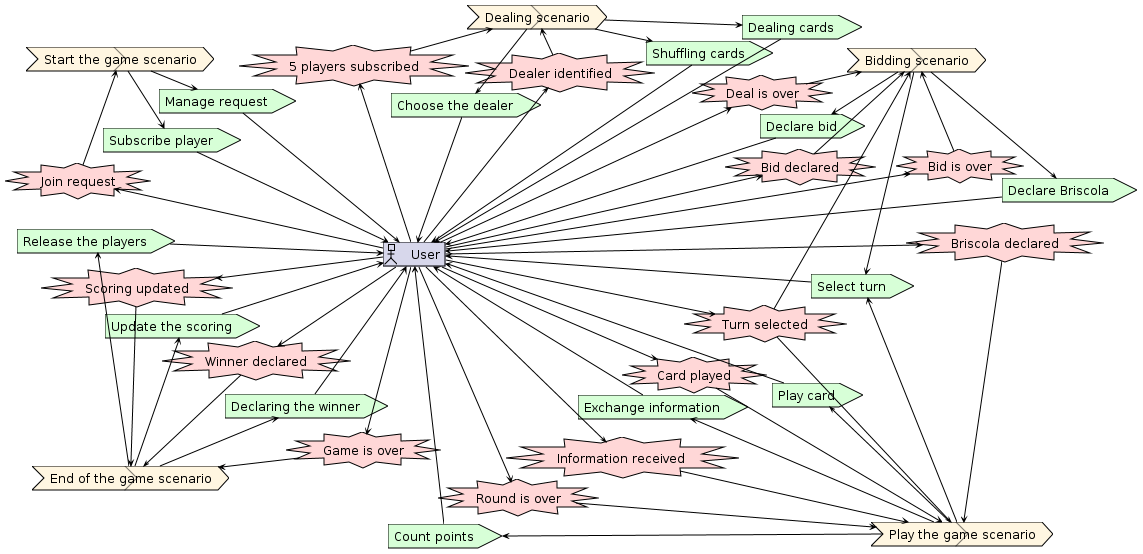
\includegraphics[keepaspectratio,scale=0.3]{pdt/images/system_specification/analysis_overview.png}
  \end{center}
}

\frame{
  \frametitle{Scenarios Diagram}

  \begin{center}
    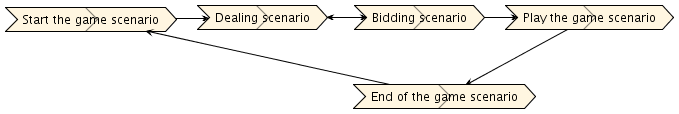
\includegraphics[keepaspectratio,scale=0.4]{pdt/images/system_specification/scenarios.png}
  \end{center}
}

\frame{
  \frametitle{Goals Overview Diagram}

  \begin{center}
    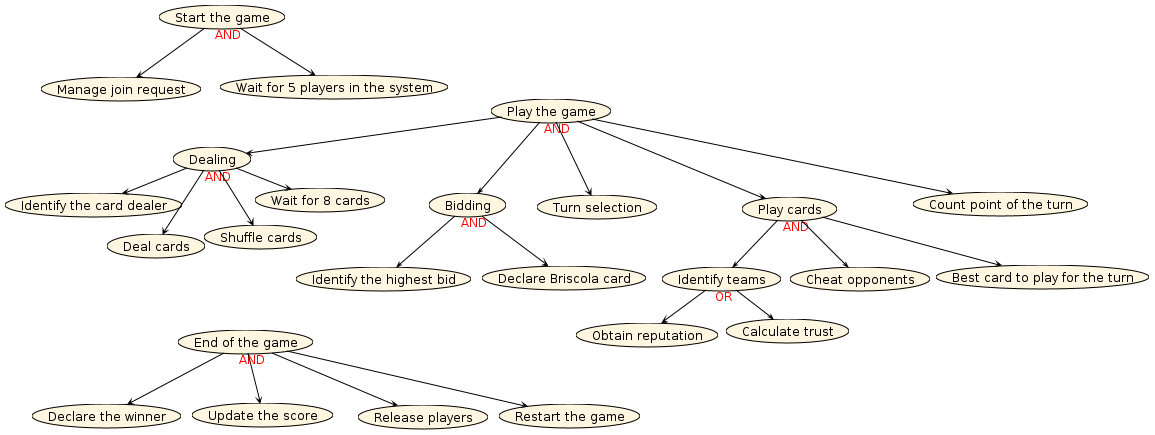
\includegraphics[keepaspectratio,scale=0.35]{pdt/images/system_specification/goal_overview.png}
  \end{center}
}

\frame{
  \frametitle{System Roles Diagram}

  ............ to be split into two subfigure with gimp

  \begin{center}
    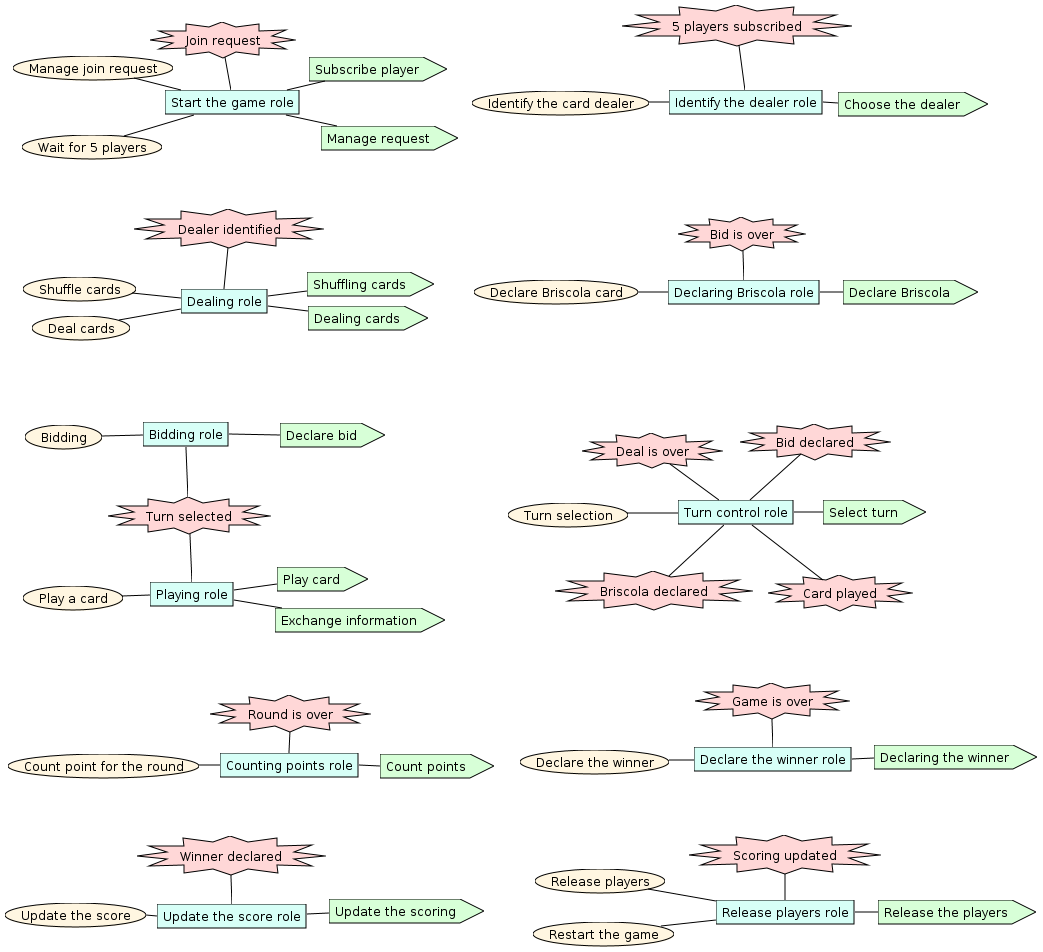
\includegraphics[keepaspectratio,scale=0.3]{pdt/images/system_specification/system_roles.png}
  \end{center}
}

\part{High-level/Architectural Design}
\frame{\partpage}

\frame{
  \frametitle{High-level/Architectural Specification}

  \begin{itemize}
    \item Data coupling diagram: links roles to data
    \item Agent-role grouping diagram: group the roles into agent types
    \item Agent acquaintance diagram: how agents interact with each's other
    \item System overview diagram: all agents in the system, along with their interface and interaction
  \end{itemize}
}

\frame{
  \frametitle{Data Coupling Diagram}

  \begin{center}
    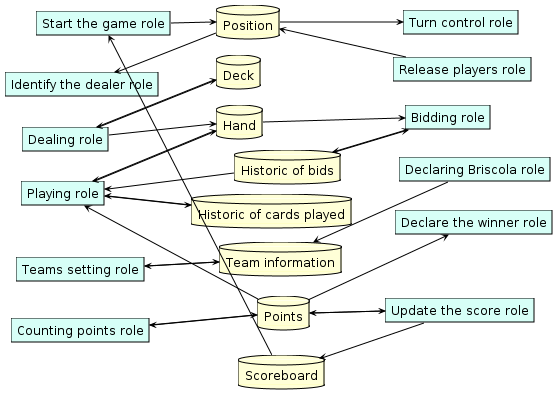
\includegraphics[keepaspectratio,scale=0.4]{pdt/images/architectural_design/data_coupling.png}
  \end{center}
}

\frame{
  \frametitle{Agent-Role Grouping Diagram}

  \begin{center}
    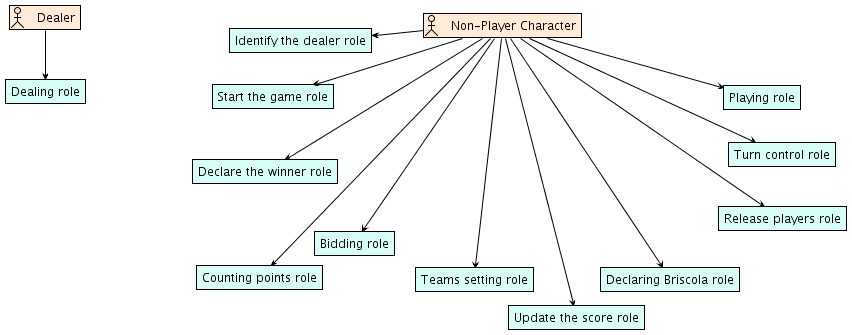
\includegraphics[keepaspectratio,scale=0.35]{pdt/images/architectural_design/aget-role_grouping.png}
  \end{center}
}

\frame{
  \frametitle{Agent Acquaintance Diagram}

  \begin{center}
    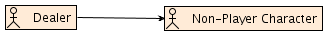
\includegraphics[keepaspectratio,scale=0.4]{pdt/images/architectural_design/agent_acquaintance.png}
  \end{center}
}

\frame{
  \frametitle{System Overview Diagram}

  \begin{center}
    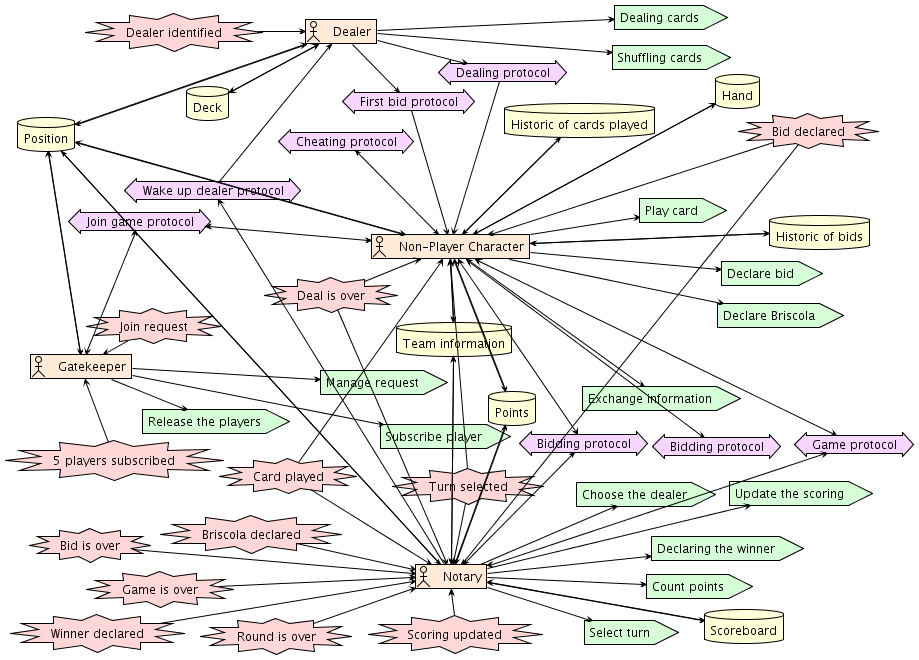
\includegraphics[keepaspectratio,scale=0.3]{pdt/images/architectural_design/system_overview.png}
  \end{center}
}

\frame[allowframebreaks]{
  \frametitle{Protocols}

  \begin{center}
  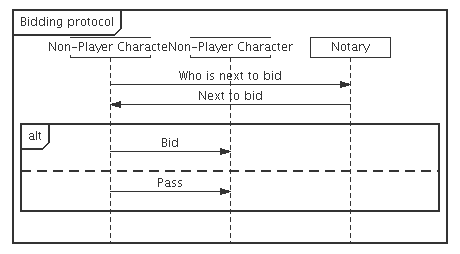
\includegraphics[keepaspectratio,scale=0.3]{pdt/images/protocols/Bidding_protocol.png}
  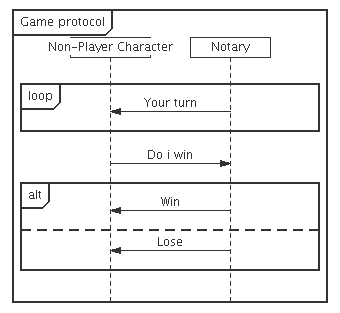
\includegraphics[keepaspectratio,scale=0.3]{pdt/images/protocols/Game_protocol.png}\\
  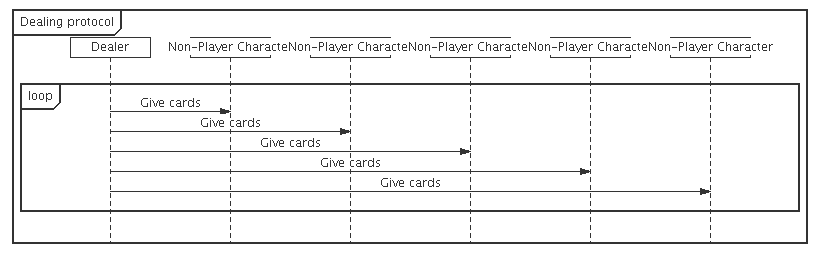
\includegraphics[keepaspectratio,scale=0.3]{pdt/images/protocols/Dealing_protocol.png}\\
  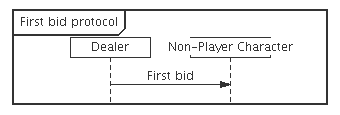
\includegraphics[keepaspectratio,scale=0.35]{pdt/images/protocols/First_bid_protocol.png}
  
\includegraphics[keepaspectratio,scale=0.35]{pdt/images/protocols/Wake_up_dealer_protocol.png}\\
  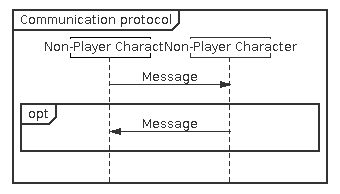
\includegraphics[keepaspectratio,scale=0.35]{pdt/images/protocols/Communication_protocol.png}
  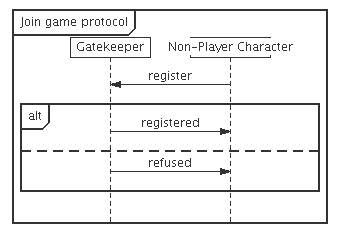
\includegraphics[keepaspectratio,scale=0.35]{pdt/images/protocols/Join_game_protocol.png}\\
  \end{center}

}

\part{Detailed Design}
\frame{\partpage}

\frame{
  \frametitle{Detailed Design}

  \begin{itemize}
    \item Agent overview diagrams: internals of agents
    \item Capability overview diagrams: internals of a capability in terms of plans or sub-capabilities and messages
  \end{itemize}
}

\frame{
  \frametitle{Agent Overview Diagram: gatekeeper agent}
  
  \begin{center}
    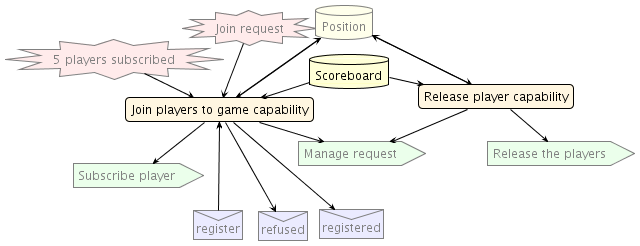
\includegraphics[keepaspectratio,scale=0.4]{pdt/images/detailed_design/gatekeeper_overview_diagram.png}
  \end{center}
}

\frame{
  \frametitle{Capability Overview Diagram: gatekeeper agent}
  \begin{center}
 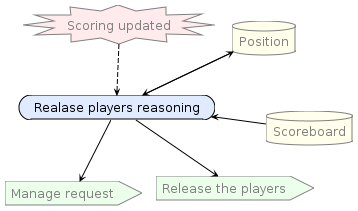
\includegraphics[keepaspectratio,scale=0.4]{pdt/images/detailed_design/release_player_capability_overview_diagram.png}
 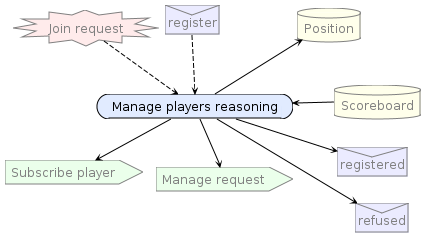
\includegraphics[keepaspectratio,scale=0.4]{pdt/images/detailed_design/join_players_capability_overview_diagram.png}
  \end{center}
}

\frame{
  \frametitle{Agent Overview Diagram: notary agent}
  
  \begin{center}
  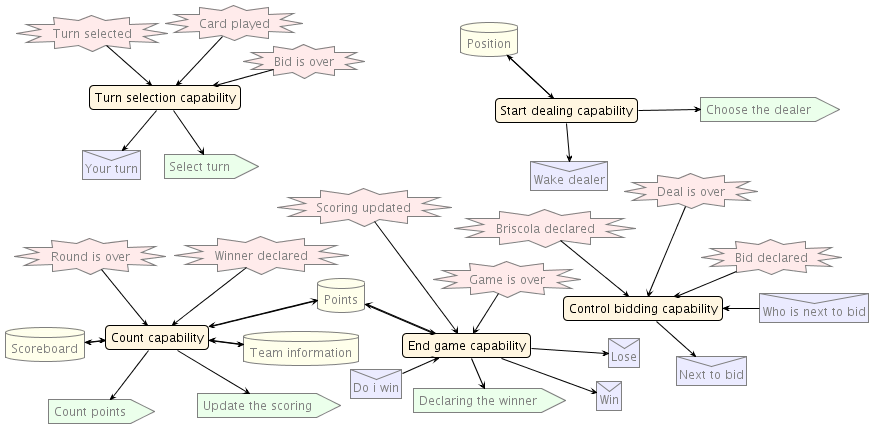
\includegraphics[keepaspectratio,scale=0.35]{pdt/images/detailed_design/notary_overview_diagram.png}
  \end{center}
}

\frame[allowframebreaks]{
  \frametitle{Capability Overview Diagram: notary agent}
  
  \begin{center}
  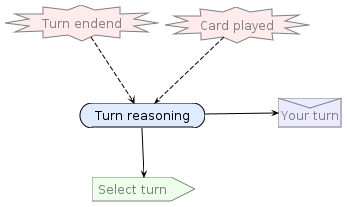
\includegraphics[keepaspectratio,scale=0.4]{pdt/images/detailed_design/turn_selection_capability_overview_diagram.png}
  
\includegraphics[keepaspectratio,scale=0.4]{pdt/images/detailed_design/end_the_game_capability_overview_diagram.png}\\
  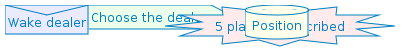
\includegraphics[keepaspectratio,scale=0.4]{pdt/images/detailed_design/start_dealing_capability_overview_diagram.png}
  
\includegraphics[keepaspectratio,scale=0.4]{pdt/images/detailed_design/control_bidding_capability_overview_diagram.png}\\
  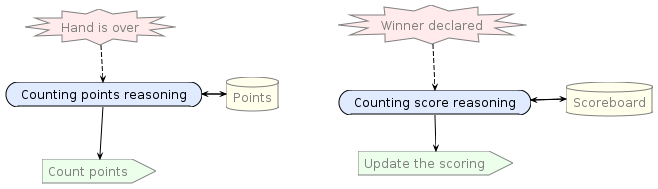
\includegraphics[keepaspectratio,scale=0.4]{pdt/images/detailed_design/count_points_capability_overview_diagram.png}
  \end{center}
}

\frame{
  \frametitle{Agent Overview Diagram: dealer agent}
  
  \begin{center}
  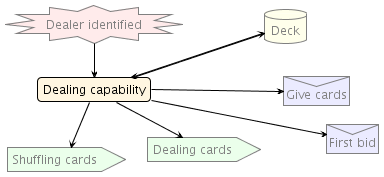
\includegraphics[keepaspectratio,scale=0.4]{pdt/images/detailed_design/dealer_overview_diagram.png}
  \end{center}
}

\frame{
  \frametitle{Capability Overview Diagram: dealer agent}
  
  \begin{center}
  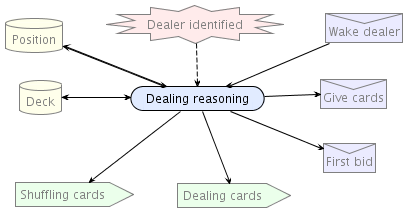
\includegraphics[keepaspectratio,scale=0.4]{pdt/images/detailed_design/dealing_capability_overview_diagram.png}
  \end{center}
}

\frame{
  \frametitle{Agent Overview Diagram: non-player-character agent}
  
  \begin{center}
  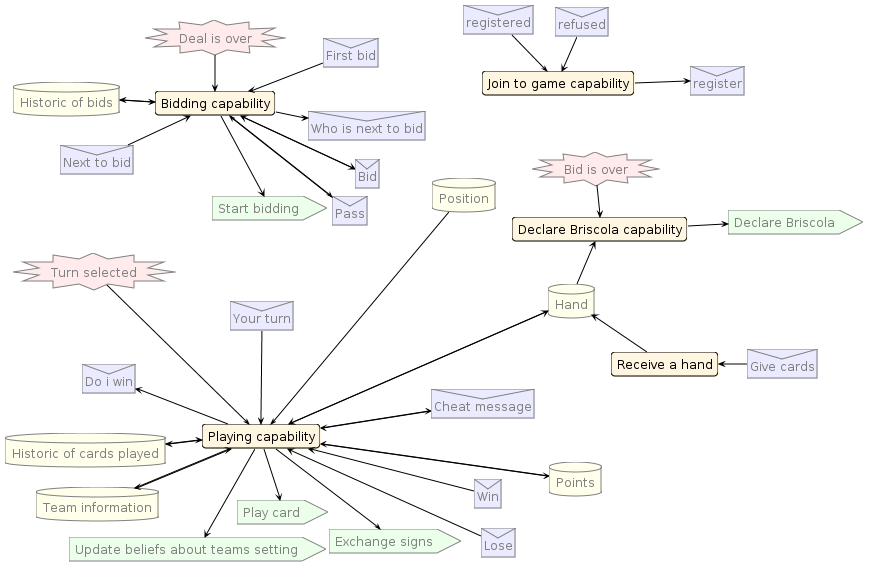
\includegraphics[keepaspectratio,scale=0.35]{pdt/images/detailed_design/non-player_character_overview_diagram.png}
  \end{center}
}

\frame[allowframebreaks]{
  \frametitle{Capability Overview Diagram: non-player-character agent}
  
  \begin{center}
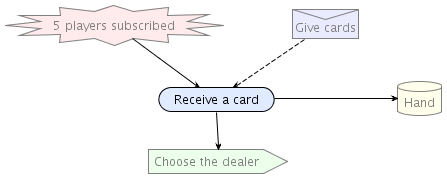
\includegraphics[keepaspectratio,scale=0.4]{pdt/images/detailed_design/receive_a_hand_capability_overview_diagram.png}
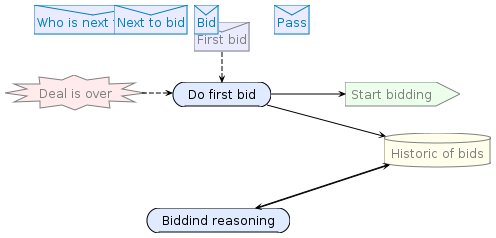
\includegraphics[keepaspectratio,scale=0.4]{pdt/images/detailed_design/bidding_capability_overview_diagram.png}\\
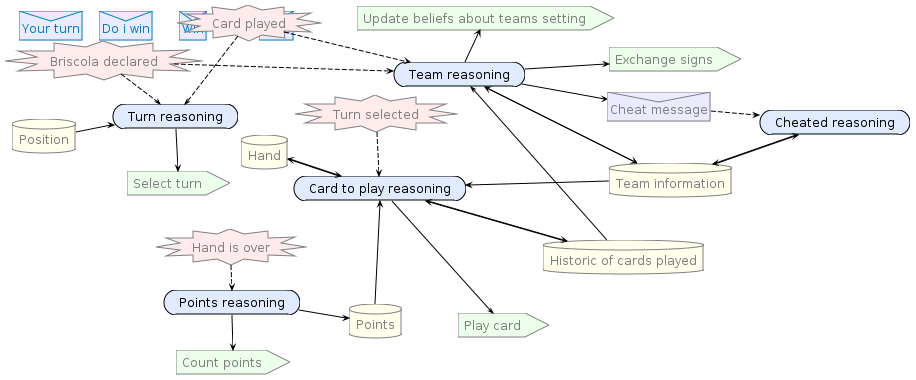
\includegraphics[keepaspectratio,scale=0.4]{pdt/images/detailed_design/playing_capability_overview_diagram.png}\\
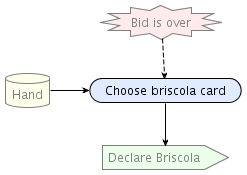
\includegraphics[keepaspectratio,scale=0.4]{pdt/images/detailed_design/declare_briscola_capability_overview_diagram.png}
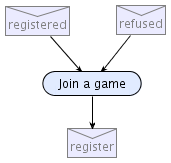
\includegraphics[keepaspectratio,scale=0.4]{pdt/images/detailed_design/join_to_game_capability_overview_diagram.png}
  \end{center}
}

\part{Prototype}
\frame{\partpage}

\frame{
  \frametitle{Prototype}
  \begin{itemize}
    \item Environment is a Java class
    \item Agents are implemented in 2APL 
    \item A GUI has been implemented
    \item Agent strategies are straight forward
  \end{itemize}
}

\part{Demo}
\frame{\partpage}

\part{Conclusions}
\frame{\partpage}

\frame{
  \frametitle{Conclusion: the good and the bad}

  \begin{columns}
    \begin{column}{0.5\textwidth}
  Good:
      \begin{itemize}
        \item Powerful mix of declarative (Prolog) and imperative programming style (Java)
        \item JADE
      \end{itemize}
    \end{column}
    \begin{column}{0.5\textwidth}
  Bad:
     \begin{itemize}
      \item Lack of library to support agent side development
      \item Lack of a manual and examples
      \item Platform not at industry level 
     \end{itemize}
    \end{column}
  \end{columns}
}


\begin{frame}{Bibliography}
\nocite{*}
\bibliographystyle{plain}
\bibliography{bc-pres}
\end{frame}

\end{document}
